\documentclass[tikz,border=6pt]{standalone}
\usepackage{xcolor}
\usepackage{tikz}
\usetikzlibrary{calc,positioning}

% --- Colors (approximate) ---
\definecolor{EBlue}{HTML}{1565C0}
\definecolor{LeftFill}{HTML}{CFE8FF}
\definecolor{MPink}{HTML}{D81B60}
\definecolor{RightFill}{HTML}{FFD1B5}
\definecolor{DarkOval}{HTML}{3F4C97}
\definecolor{BroadTxt}{HTML}{5C6BC0}

% --- Styles ---
\tikzset{
  vennA/.style={draw=EBlue, line width=1.1pt, fill=LeftFill, fill opacity=0.42},
  vennB/.style={draw=MPink, line width=1.1pt, fill=RightFill, fill opacity=0.42},
  innerband/.style={fill=DarkOval, draw=none},
  labelL/.style={font=\small, text=EBlue},
  labelR/.style={font=\small, text=MPink, align=center},
  labelMid/.style={font=\small, text=BroadTxt},
  title/.style={font=\normalsize}
}

\begin{document}
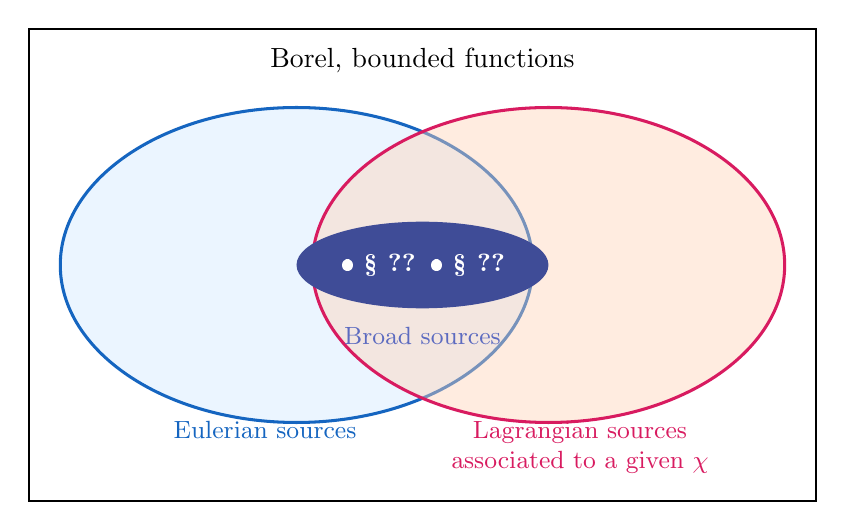
\begin{tikzpicture}[x=1cm,y=1cm,inner sep=1pt,outer sep=0pt]
  % Canvas frame (10 x 6 cm)
  \draw[black, line width=0.8pt] (0,0) rectangle (10,6);

  % Title
  \node[title] at (5,5.6) {Borel, bounded functions};

  % Two main ellipses
  \path[vennA] (3.4,3.0) ellipse [x radius=3.0, y radius=2.0];
  \path[vennB] (6.6,3.0) ellipse [x radius=3.0, y radius=2.0];

  % Central narrow oval band in the overlap
  \path[innerband] (5.0,3.0) ellipse [x radius=1.6, y radius=0.55];

  % Texts inside the band (white for contrast)
  \node[font=\small\bfseries, text=white, anchor=east] at (4.95,3.0) {\textbullet\ \S\ ??};
  \node[font=\small\bfseries, text=white, anchor=west] at (5.05,3.0) {\textbullet\ \S\ ??};

  % Overlap caption
  \node[labelMid, anchor=north] at (5.0,2.25) {Broad sources};

  % Bottom labels
  \node[labelL, anchor=north] at (3.0,1.05) {Eulerian sources};
  \node[labelR, anchor=north] at (7.0,1.05) {Lagrangian sources\\associated to a given $\chi$};
\end{tikzpicture}
\end{document}